% Created 2023-11-02 Thu 21:59
% Intended LaTeX compiler: pdflatex
\documentclass[11pt]{article}
\usepackage[utf8]{inputenc}
\usepackage[T1]{fontenc}
\usepackage{graphicx}
\usepackage{longtable}
\usepackage{wrapfig}
\usepackage{rotating}
\usepackage[normalem]{ulem}
\usepackage{amsmath}
\usepackage{amssymb}
\usepackage{capt-of}
\usepackage{hyperref}
\usepackage{graphicx, siunitx}
\graphicspath{ {./images/} }
\author{Hankertrix}
\date{\today}
\title{Physics Capacitance \& DC Circuits Cheat Sheet}
\hypersetup{
 pdfauthor={Hankertrix},
 pdftitle={Physics Capacitance \& DC Circuits Cheat Sheet},
 pdfkeywords={},
 pdfsubject={},
 pdfcreator={Emacs 29.1 (Org mode 9.6.6)}, 
 pdflang={English}}
\begin{document}

\maketitle
\setcounter{tocdepth}{2}
\tableofcontents

\newpage

\section{Definitions}
\label{sec:org8ec3c2d}

\subsection{Resistance}
\label{sec:org8d38481}
Resistance is defined as:
\[R = \frac{V}{I}\]

Where:
\begin{itemize}
\item \(I\) is the current passing through the resistor
\item \(V\) is the potential difference, or the voltage, across the resistor
\end{itemize}

\subsection{Ohm's law}
\label{sec:orged3751e}
Ohm's law states that the ratio of the potential difference \(V\) across a device to the current \(I\) passing through it is a constant. Essentially, Ohm's law states that resistance \(R\) is a constant.

\subsubsection{Ohmic resistor}
\label{sec:org275549a}
An ohmic resistor, such as a typical metal wire, is a resistor that obeys Ohm's law. The potential difference across the resistor is proportional to the current passing through the resistor at a given temperature.

\subsubsection{Non-ohmic resistor}
\label{sec:orgb82f3bb}
For non-ohmic resistors, the graph is typically a curve and hence it is incorrect to say that \(\frac{1}{R}\) is the \textbf{slope} of an \(I-V\) graph.

\subsection{Electromotive force (\(emf\) or \(\varepsilon\))}
\label{sec:org34e0e60}
The electromotive force is defined as the electric potential produced by a source, such as an electrochemical cell, i.e. a battery, or a changing magnetic field. The calculation of the electromotive force is the same as the potential difference.
\\[0pt]

Electromotive force is also the work done per unit charge:
\[\varepsilon = \frac{W}{Q}\]

\begin{itemize}
\item \(W\) is the work done by a source
\item \(Q\) is the total charge
\end{itemize}

\subsection{Internal resistance of a battery}
\label{sec:org85ae169}
The internal resistance of a battery is given as:
\[V_{ab} = \varepsilon - Ir\]

Where:
\begin{itemize}
\item \(V_{ab}\) is the terminal voltage of the source with internal resistance
\item \(\varepsilon\) is the electromotive force of the source
\item \(I\) is the current through the source
\item \(r\) is the internal resistance of the source
\end{itemize}

\subsection{Kirchhoff's current rule}
\label{sec:org8412b02}
Kirchhoff's current rule states that the sum of the currents into any junction is equal to 0.
\[\sum I = 0\]

\subsection{Kirchhoff's voltage rule}
\label{sec:org4c4e845}
Kirchhoff's voltage rule states that the sum of the potential differences around any closed loop is equal to 0.
\[\sum V = 0\]

\newpage

\subsection{Power}
\label{sec:orgcb8b943}
The power of a circuit is defined as follows:
\[P = V_{ab} I\]

Where:
\begin{itemize}
\item \(P\) is the power delivered to or extracted from a circuit element
\item \(V_{ab}\) is the voltage across the circuit element
\item \(I\) is the current in the circuit element
\end{itemize}

Power is can also be defined using resistance:
\[P = I^2 R = \frac{V_{ab}^2}{R}\]

Where:
\begin{itemize}
\item \(P\) is the power delivered to or extracted from a circuit element
\item \(V_{ab}\) is the voltage across the circuit element
\item \(I\) is the current in the circuit element
\item \(R\) is the resistance of the circuit element
\end{itemize}

\subsection{Capacitance (\(C\)) (SI Unit: \(\unit{F}\))}
\label{sec:org3243b41}
The capacitance \(C\) of a capacitor is defined as the ratio of the magnitude of the charge \(Q\) on either conductor to the magnitude of the potential difference between the conductors \(V_{ab}\).

\[C = \frac{Q}{V_{ab}}\]

Where:
\begin{itemize}
\item \(C\) is the capacitance of a capacitor
\item \(Q\) is the magnitude of charge on each conductor
\item \(V_{ab}\) is the potential difference between conductors (\(a\) has charge \(+Q\) and \(b\) has charge \(-Q\))
\end{itemize}

Thus, a capacitor with large capacitance is one which can hold a huge charge even when the potential difference across the two plates is small. The SI unit for capacitance is farad (\(\unit{F}\)).

\subsubsection{Capacitance of a parallel plate capacitor}
\label{sec:org3c64e08}
\[C = \frac{Q}{V_{ab}} = \frac{\varepsilon_0 A}{d}\]

Where:
\begin{itemize}
\item \(C\) is the capacitance of a parallel-plate capacitor in vacuum
\item \(Q\) is the magnitude of the charge on each plate
\item \(V_{ab}\) is the potential difference between the two plates
\item \(\varepsilon_0\) is the permittivity of vacuum
\item \(A\) is the area of each plate
\item \(d\) is the distance between the two plates
\end{itemize}

\subsubsection{Capacitance of a conducting sphere}
\label{sec:org793408a}
\[C = 4 \pi \varepsilon_0 r\]

Where:
\begin{itemize}
\item \(C\) is the capacitance of the conducting sphere
\item \(\varepsilon_0\) is the permittivity of vacuum
\item \(r\) is the radius of the sphere
\end{itemize}

\subsubsection{Capacitance of a co-axial cylindrical capacitor}
\label{sec:org13c5f14}
\[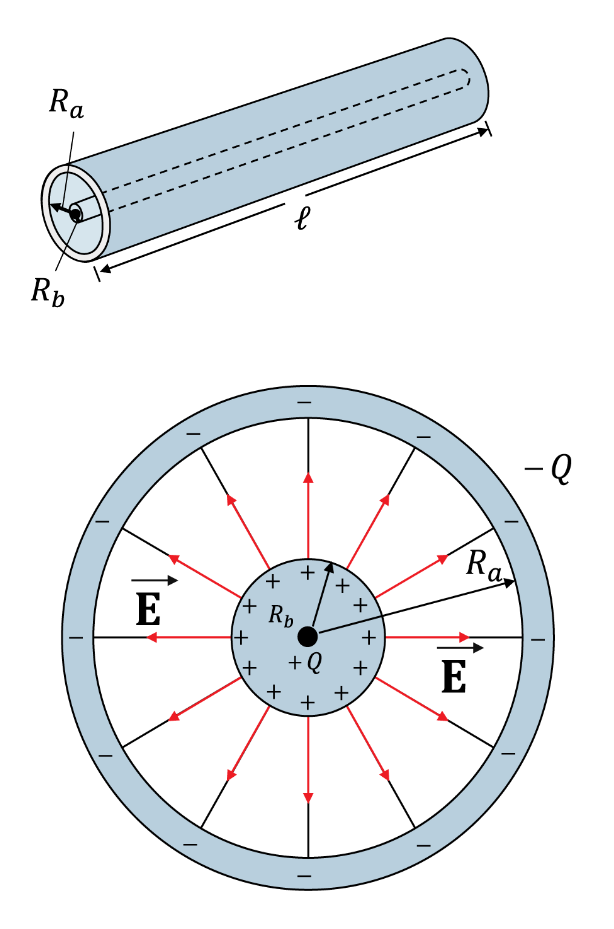
\includegraphics[scale = 0.7]{co-axial-cyclindrical-capacitor}\]
\[C = \frac{2 \pi \varepsilon_0 L}{\ln \left| \frac{R_a}{R_b} \right|}\]

Where:
\begin{itemize}
\item \(C\) is the capacitance of the co-axial cylindrical capacitor
\item \(\varepsilon_0\) is the permittivity of vacuum
\item \(L\) is the length of the capacitor
\item \(R_a\) is the radius of the \textbf{inner} surface of the \textbf{larger outer} cylinder
\item \(R_b\) is the radius of the \textbf{smaller} cylinder on the inside of the capacitor
\end{itemize}

\subsection{Dielectric}
\label{sec:org8b654db}
Dielectric is just another word for an insulator.

\subsection{Dielectric breakdown}
\label{sec:org4782cd3}
Dielectric breakdown refers to the phenomenon where the dielectric or the insulator becomes a conductor due to a strong electric field.

\subsection{Dielectric strength}
\label{sec:orgfc4789c}
Dielectric strength refers to the maximum electric field a dielectric or insulator can handle before it becomes a conductor.


\section{Formulas}
\label{sec:orgacc980c}

\subsection{Resistors in series}
\label{sec:org88c1a85}
\begin{itemize}
\item The resistors have the same current \(I\).
\item Their potential differences add.
\end{itemize}
\[R_{eq} = R_1 + R_2 + R_3 + \cdots\]

Where:
\begin{itemize}
\item \(R_{eq}\) is the equivalent resistance of the resistors in series
\item \(R_n\), where \(n = 1, 2, 3, \ldots\), is the resistances of the individual resistors
\end{itemize}

\subsection{Resistors in parallel}
\label{sec:org2082456}
\begin{itemize}
\item The resistors have the same potential \(V\).
\item The current passing through each resistor is dependent on its resistance: \(I_1 = \frac{V}{R_1}\)
\end{itemize}
\[\frac{1}{R_{eq}} = \frac{1}{R_1} + \frac{1}{R_2} + \frac{1}{R_3} + \cdots\]

Where:
\begin{itemize}
\item \(R_{eq}\) is the equivalent resistance of the resistors in series
\item \(R_n\), where \(n = 1, 2, 3, \ldots\), is the resistances of the individual resistors
\end{itemize}

\subsection{Capacitors in series}
\label{sec:org60f4e7c}
\begin{itemize}
\item The capacitors have the same charge \(Q\).
\item Their potential differences add.
\end{itemize}

\[\frac{1}{C_{eq}} = \frac{1}{C_1} + \frac{1}{C_2} + \frac{1}{C_3} + \cdots\]

Where:
\begin{itemize}
\item \(C_{eq}\) is the equivalent capacitance of the capacitors in series
\item \(C_n\), where \(n = 1, 2, 3, \ldots\), is the capacitances of the individual capacitors
\end{itemize}

\subsection{Capacitors in parallel}
\label{sec:orgc77ad3f}
\begin{itemize}
\item The capacitors have the same potential \(V\).
\item The charge on each capacitor depends on its capacitance: \(Q_1 = C_1 V\)
\end{itemize}
\[C_{eq} = C_1 + C_2 + C_3 + \cdots\]

Where:
\begin{itemize}
\item \(C_{eq}\) is the equivalent capacitance of the capacitors in parallel
\item \(C_n\), where \(n = 1, 2, 3, \ldots\), is the capacitances of the individual capacitors
\end{itemize}

\subsection{Potential energy stored in a capacitor}
\label{sec:orgb2bdbdc}
\begin{align*}
U &= \frac{Q^2}{2C} \\
&= \frac{1}{2} CV^2 \\
&= \frac{1}{2} QV
\end{align*}

Where:
\begin{itemize}
\item \(U\) is the potential energy stored in a capacitor
\item \(Q\) is the magnitude of charge on each plate
\item \(C\) is the capacitance of the capacitor
\item \(V\) is the potential difference between plates
\end{itemize}

\subsection{Electric energy density in a vacuum}
\label{sec:org77eb22d}
\[u = \frac{1}{2} \varepsilon_0 E^2\]

Where:
\begin{itemize}
\item \(u\) is the electric energy density in a vacuum
\item \(\varepsilon_0\) is the permittivity of vacuum
\item \(E\) is the magnitude of the electric field
\end{itemize}

\subsection{Electric energy density in the presence of a dielectric or insulator}
\label{sec:org2203d05}
\begin{align*}
u &= \frac{1}{2} \varepsilon_r \varepsilon_0 E^2 \\
&= \frac{1}{2} K \varepsilon_0 E^2 \\
&= \frac{1}{2} \varepsilon E^2
\end{align*}

Where:
\begin{itemize}
\item \(u\) is the electric energy density in vacuum
\item \(\varepsilon_0\) is the permittivity of vacuum
\item \(\varepsilon_r\) is the relative permittivity of the dielectric or insulator
\item \(K\) is the dielectric constant
\item \(E\) is the magnitude of the electric field
\item \(\varepsilon\) is the permittivity and it is equal to \(K \varepsilon_0\)
\end{itemize}

\newpage

\subsection{Capacitance with a dielectric}
\label{sec:org567cbee}
\begin{align*}
C &= KC_0 \\
&= K \varepsilon_0 \frac{A}{d} \\
&= \varepsilon \frac{A}{d}
\end{align*}

Where:
\begin{itemize}
\item \(C\) is the capacitance of a parallel-plate capacitor with dielectric between the plates
\item \(K\) is the dielectric constant
\item \(C_0\) is the capacitance without the dielectric
\item \(\varepsilon_0\) is the permittivity of vacuum
\item \(A\) is the area of each plate
\item \(d\) is the distance between the plates
\item \(\varepsilon\) is the permittivity and it is equal to \(K \varepsilon_0\)
\end{itemize}

\subsection{Gauss' law in dielectrics}
\label{sec:org0aea28a}
\[\oint K \vec{E} \cdot \, d \vec{A} = \frac{Q_{encl-free}}{\varepsilon_0}\]

Where:
\begin{itemize}
\item \(\oint K \vec{E} \cdot \, d \vec{A}\) is the surface integral of \(K \vec{E}\) over a closed surface
\item \(K\) is the dielectric constant
\item \(Q_{encl-free}\) is the total free charge enclosed by the surface
\item \(\varepsilon_0\) is the permittivity of vacuum
\end{itemize}

\newpage

\subsection{Charging a capacitor}
\label{sec:org9bb589c}

\subsubsection{Capacitor charge}
\label{sec:org2d46a43}
\begin{align*}
q &= C \mathcal{E} (1 - e^{- \frac{t}{RC}}) \\
&= Q_f(1 - e^{-\frac{t}{RC}})
\end{align*}

Where:
\begin{itemize}
\item \(q\) is the capacitor charge
\item \(R\) is the resistance
\item \(C\) is the capacitance
\item \(\mathcal{E}\) is the electromotive force of the battery
\item \(t\) is the time since the switch is closed
\item \(Q_f\) is the final capacitor charge, which is equal to \(C \mathcal{E}\)
\end{itemize}

\subsubsection{Resulting current in the circuit}
\label{sec:orgfbb9ab2}
\begin{align*}
i &= \frac{dq}{dt} \\
&= \frac{\mathcal{E}}{R} e^{-\frac{t}{RC}} \\
&= I_0 e^{-\frac{t}{RC}}
\end{align*}

Where:
\begin{itemize}
\item \(i\) is the current in the circuit
\item \(\frac{dq}{dt}\) is the rate of change of capacitor charge
\item \(\mathcal{E}\) is the electromotive force of the battery
\item \(R\) is the resistance
\item \(C\) is the capacitance
\item \(t\) is the time since the switch is closed
\item \(I_0\) is the initial current, which is equal to \(\frac{\mathcal{E}}{R}\)
\end{itemize}

\subsection{Discharging a capacitor}
\label{sec:org96e3d74}

\subsubsection{Capacitor charge}
\label{sec:org718f5ea}
\[q = Q_0 e^{-\frac{t}{RC}}\]

Where:
\begin{itemize}
\item \(q\) is the capacitor charge
\item \(Q_0\) is the initial capacitor charge
\item \(t\) is the time since the switch is closed
\item \(R\) is the resistance
\item \(C\) is the capacitance
\end{itemize}

\subsubsection{Resulting current in the circuit}
\label{sec:org8297bc2}
\begin{align*}
i &= \frac{dq}{dt} \\
&= - \frac{Q_0}{RC} e^{-\frac{t}{RC}} \\
&= I_0 e^{- \frac{t}{RC}}
\end{align*}

Where:
\begin{itemize}
\item \(i\) is the current in the circuit due to the capacitor discharging
\item \(\frac{dq}{dt}\) is the rate of change of capacitor charge
\item \(Q_0\) is the initial capacitor charge
\item \(t\) is the time since the switch is closed
\item \(R\) is the resistance
\item \(C\) is the capacitance
\item \(I_0\) is the initial current, which is equal to \(- \frac{Q_0}{RC}\)
\end{itemize}


\section{Sign conventions and procedures in Kirchhoff's rules}
\label{sec:org8f1df81}

\subsection{Procedures for applying Kirchhoff's rules}
\label{sec:org6670192}
\begin{enumerate}
\item Give arbitrary (guessed) directions for current. Indicate them in the circuit.
\item Apply Kirchhoff's current rule at junctions.
\item Choose any closed loop in the circuit to apply Kirchhoff's voltage rule.
\item The changes in the potential are determined by the direction of "travel" as you trace around the loop, and the terminal potential differences across the devices.
\item Upon arriving at a solution, if the current is positive, it means the guessed direction was correct. If the current is negative, it means the correct direction is opposite to the guess. The rules are self-consistent in this way.
\end{enumerate}

\subsection{Important notes}
\label{sec:orgbe70d47}
\begin{itemize}
\item For a battery, the terminal potentials are determined by the polarity of the terminals.
\item For a resistor, the terminal potentials are determined by the direction of current flow.
\item When the current passes through a component that is from negative to positive, add the potential difference across that component. This is because the \textbf{potential is increasing} from the negative terminal to the positive terminal. In simpler terms: \((- \rightarrow +) \text{ means } + V\).
\item When the current passes through a component that is from positive to negative, subtract the potential difference across that component. This is because the \textbf{potential is decreasing} from the positive terminal to the negative terminal. In simpler terms: \((+ \rightarrow -) \text{ means } - V\).
\end{itemize}

\newpage

\section{Capacitors in circuits}
\label{sec:org608bc03}
\begin{itemize}
\item When the capacitor is \textbf{uncharged}, or has \textbf{just begun charging}, the capacitor acts as a \textbf{regular metal wire}, or a \textbf{short circuit}.
\item When the capacitor is \textbf{fully charged}, the capacitor acts like a \textbf{break in the circuit} and effectively has \textbf{infinite resistance}.
\item When two charged capacitors are connected to each other, \textbf{positive plate to positive plate}, the charges will transfer until the \textbf{potential difference is the same} for both capacitors.
\end{itemize}

\newpage

\section{Voltmeters and ammeters in a DC circuit}
\label{sec:org7470a63}
\[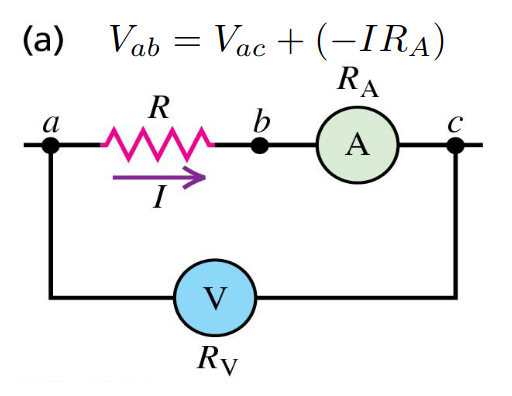
\includegraphics{voltmeter-and-ammeter-configuration-1}\]
The reading of the voltmeter above is an over-estimate, as it includes the potential difference across the ammeter. Ideally, the resistance of an ammeter is zero, so as not to distort the current it aims to measure.

\[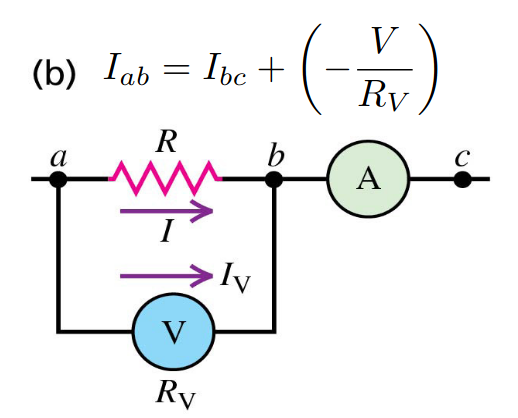
\includegraphics{voltmeter-and-ammeter-configuration-2}\]
The reading of the ammeter above is an over-estimate. It includes the current drawn by the voltmeter. Ideally, the resistance of a voltmeter is infinite, so as not to draw any current which will distort the potential difference it aims to measure.


\section{Electrostatic equilibrium}
\label{sec:org680effb}
For a conductor that is in electrostatic equilibrium:
\begin{enumerate}
\item The electric field is zero everywhere inside the conductor.
\item The surface of the conductor is an equipotential surface.
\item If the conductor is isolated, any net charge resides on the surface.
\item The electric field near the surface of the conductor is normal (\(90^{\circ}\)) to the surface.
\item For irregularly shaped conductors, the surface charge density is greatest at regions where the radius of curvature of the surface is the smallest.
\item If excess charges are added to the conductor, the excess charges move to the surfaces of the conductor until a new equilibrium is established where the electric field is zero within the conductor again.
\end{enumerate}


\section{Energy deficit}
\label{sec:org444f116}
A battery puts out energy \(QV_b\) in the process of charging the capacitor to equilibrium at battery voltage \(V_b\). However, \textbf{only half} (\(\frac{QV_b}{2}\)) is finally stored on the capacitor. The energy is lost in the form of heat in high resistance charging, and is lost in the form of electromagnetic radiation in low resistance charging. This \textbf{energy loss} is always \textbf{half} of the \textbf{work done} by the battery.
\end{document}